\documentclass[letterpaper,11pt]{article}
\usepackage[spanish]{babel}
\usepackage{graphicx}
\usepackage{url}
\usepackage[utf8]{inputenc}
\usepackage{listings}
\usepackage{caption}
\usepackage{algorithmic}
\usepackage{caption}
\usepackage{amsthm}
\setlength{\parindent}{1em}
\newtheorem*{definicion}{Definici\'on}

\begin{document}

\begin{figure}[htp]
  \centering
  
\includegraphics[scale=0.1]{logoUSB.png}
\end{figure}

\begin{center}
  \textbf{UNIVERSIDAD SIM\'ON BOL\'IVAR}\\
  Ingenier\'ia de la Computaci\'on\\
  Dise\~no de Algoritmos II - CI-5652
\end{center}
\begin{center}	
  \vspace{2in}
  \textsf{\begin{Large}\bf One-Dimensional Cutting Stock Problem (CSP)\end{Large}}

\begin{Large}
3ra. Entrega
\end{Large}
      
\end{center}
\begin{center}
  \vspace{2in}
  Juan Garc\'ia 05-38207\\
  Federico Flaviani 99-31744\\
  \vspace{0.25in}	
  \today
\end{center}
\newpage

\tableofcontents
\newpage

\section{Introducci\'on}

\subsection{Breve descripci\'on del problema}

Cutting Stock Problem (CSP) o Problema de Corte y Empaquetamiento es un problema de optimizaci\'on
orientado al \'area de la programaci\'on entera, en donde el objetivo es minimizar el desperdicio generado
al cortar una serie de patrones en un \'area dada. Este problema surge regularmente en el \'area de la
industria sider\'urgica o del papel, en donde se busca disminuir las p\'erdidas monetarias por desperdicios
de material.\\

\begin{figure}[htp]
\centering
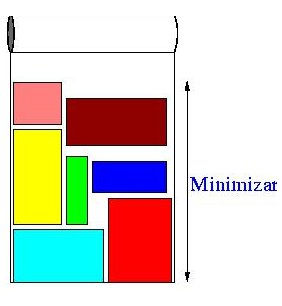
\includegraphics[scale=0.7]{faixa3.jpg}
\caption{Forma general de CSP en dos dimensiones}
\end{figure}

En CSP se dispone de un \'area la cual deseamos cortar y existen muchas maneras de representarla. Puede
ser una tela de tamaño finito en todos los sentidos, o una tela de ancho fijo con altura infinita, que es
el caso que trataremos en este proyecto. Luego se tienen una serie de formas o patrones que queremos cortar
de la mencionada tela. Dado que nuestro problema es la versi\'on unidimensional (Figura 2), las piezas que se quieren
cortar de la tela seran rectangulos con base constante igual a uno y con alturas variadas. Adem\'as no se
permitir\'a el cambio de orientaci\'on de las piezas. Instancias del problema con mas nivel de dificultad
se encuentra con la versi\'on de dos dimensiones y piezas de tamaño y formas variables, asi como en tres
dimensiones, en donde el problema se basa en optimizar la forma de empaquetar piezas en un volumen
dado, tipo un contenedor de mercancia.

\begin{figure}[htp]
\centering
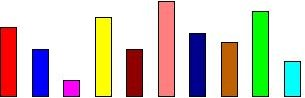
\includegraphics[scale=0.7]{Untitled.jpg}
\caption{Generalizaci\'on a cortes unidimensionales}
\end{figure}

\newpage

\section{Dise\~no}

\subsection{Modelo utilizado para representar el problema}

Como se mencion\'o anteriormente la forma en que representamos el problema es usando una tela "infinita" con
ancho fijo. Para representar la infinitud de la tela hallamos una cota superior que cubra todos los posibles
cortes que se pueden realizar, de esta forma nuestra cota superior $CS$ sera: $$ CS =  \sum_{i = 1}^{N} L_i $$ 
donde $N$ es el n\'umero de piezas a cortar y $L_i$ es el largo de la pieza $i$.\\
En nuestro programa crearemos una serie de estructuras para representar cada parte del problema, comenzando con las
piezas que queremos cortar, pasando por patrones de corte ya establecidos, los cuales representaran en
nuestro caso una soluci\'on factible.

\subsection{Estructuras y algoritmos involucrados en la aplicaci\'on}

Dentro de las principales estructuras que utilizamos, estan aquellas que nos permiten representar
un estado o soluci\'on factible. Para ellos necesitamos piezas y un patr\'on de corte, por lo tanto
se definir\'an las estrucutras \emph{Piece} y \emph{Pattern} en conjunto con su tanda de atributos
y diferentes m\'etodos.\\

En cuanto a los algoritmos utilizados, encontramos en primera instancia un algoritmo greedy que nos
permitira crear una soluci\'on inicial. Luego se aplicar\'an una serie de procedimientos con el fin de
determinar una vecindad en un cierto espacio. Para finalmente aplicar los algortimos de las diferentes
meta-heuristicas que se van a implementar para resolver el problema.\\

En primera instancia el algoritmo greedy que genera una soluci\'on inicial consistia en ir aplicando cortes sucecivos a la tela, de la manera mas eficiciente posible. Primero se ordenaban los cortes a realizar seg\'un el tamaño de mayor a menor, para comenzar\'a por la base colocando las piezas por fila. El problema de esta solucion inicial
es que siempre generaba un optimo local, por lo tanto los algoritmos de busqueda no lograban optmimizar mas alla
de lo que generaba la solucion.

Para resolver esta problem\'atica se decidi\'o no ordenar las piezas por el tama\~no, sino ir realizando
los cortes en el orden en que se iban aplicando las demandas de los clientes. Y luego de colocar lor cortes, 
se aplica una rutina de perturbaci\'on, que permite degerar mas la soluci\'on, y as\'i ayudar a las metaheur\'isticas
a encontrar una mejor soluci\'on.

\subsubsection{Clase Piece}

Esta clase representa una pieza a ser cortada de la tela. Posee un atributo, \emph{large} que representa
el largo del rectangulo a cortar. Adem\'as, como todo objeto tiene un constructor que recibe como par\'ametros un entero que representa el largo del bloque para inicializar el tama\~no del mismo en la tela. Finalmente posee un m\'etodo \emph{clone} que permite crear una copia de una pieza.

\begin{verbatim}
class Piece {
 public:
  int large;
  Piece(int);
  Piece clone();
};
\end{verbatim}

\subsubsection{Clase Pattern}

La clase \emph{Pattern} representa un patr\'on de corte de una isntancia del problema del CSP. Es decir es
una solucion factible, en donde estan posicionadas todas las piezas de corte sobre la tela. A partir de una
instancia de patter se obtienen otras instancias de la misma aplicacando los operadores de vecindad, asi como
se puede obtener el nivel de calidad de la misma, para hacer comparaciones entre un patr\'on y otro.\\

La clase tiene una serie de atributos y m\'etodos, pero dentro de los mas importantes encontramos a \emph{width} y
\emph{height} que representan el alto y ancho de la tela a cortar. \emph{num\_pieces} y \emph{pieces} son el n\'umero
de piezas y la lista que contiene a las mismas, repectivamente. Adem\'as otros atributos que modelan el area ocupada
y \'area libre, el n\'umero de lineas concretadas en el patr\'on y variables enteras que soportan la generaci\'on de las
vecindades.\\

Dentro de los m\'etodos mas importantes encontramos los constructores de clase, que permiten inicializar un patr\'on cualquiera, tambi\'en el m\'etodo \emph{vicinityNext} que permite ir generando la vecindad dinamincamente, basado en
los m\'etodos \emph{vicinityFirstLevel}, \emph{vicinitySecondLevel} y \emph{vicinityThirdLevel}, el m\'etodo \emph{perturbar} que permite pertubar una soluci\'on iniciada para aplicar la metaheuristica \emph{ILS}, entre otros m\'etodos de apoyo para hacer revision de calidad y de la funci\'on objetivo.

\begin{verbatim}
  int **paper;
  int width;
  int height;
  int heightMax;
  int num_pieces;
  list<Piece *>* pieces;
  int area_ocup;
  int area_no_ocup;
  int lines;
  
  Pattern();
  Pattern(int, int);
  Pattern(list<Piece *>, int, int);

  list<Pattern *> genVicinity();
  Pattern* vicinityOperator(int, int, int);
  void swap(int *, int, int);
  void updateRemovePaper(Piece *);
  void updateAddPaper(Piece *);
  void deleteList(list<Pattern *> *);
  Pattern* perturb();
  Pattern* clone();
  int calcHeight();
  int quality();
  void actualizar();
  void print();
  void swap();
  Pattern* addRequest(list<Piece *>);
  void addPiece(Piece *, int);
\end{verbatim}

\subsubsection{Clase Chromosome}

Esta clase representa un Cromosoma en la implementaci\'on del algoritmo Gen\'etico. Basicamente posee una matriz
que almacena las demandas de los clientes por fila, y por columna se representa una torre de piezas ubicadas por columna a lo ancho de la tela. 

\begin{figure}[htp]
\centering
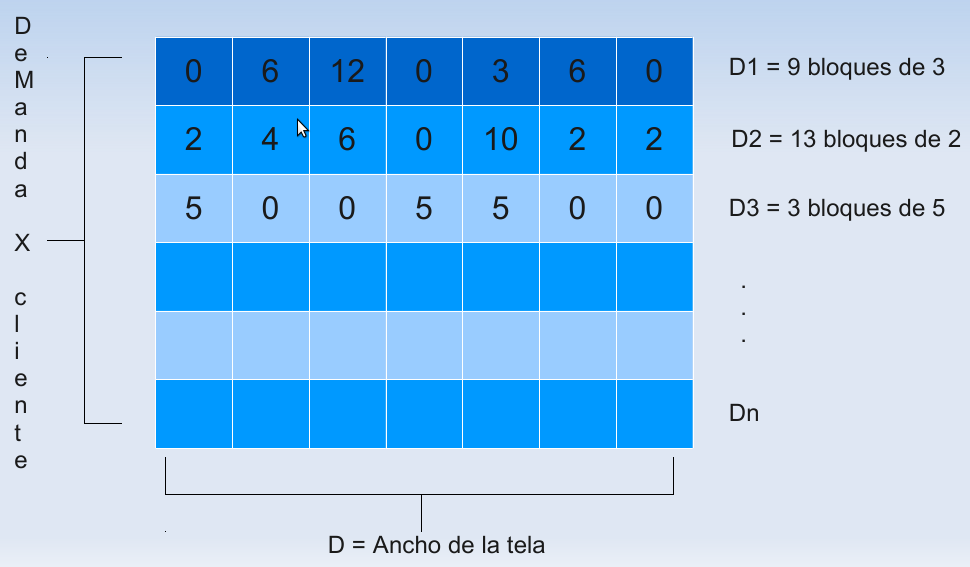
\includegraphics[scale=0.2]{ch.png}
\caption{Representaci\'on de un cromosoma}
\end{figure}

Posee otros atributos que permiten terminar de representar un cromosoma y obtener una soluci\'on factible del mismo, en referencia al problema que estamos atacando. Variables que almacenan el ancho y alto de la matriz, la altura m\'axima alcanzada, la calidad del cromosoma, el \'area ocupada por el patr\'on y las lineas generadas. De igual forma posee m\'etodos que permiten construir un nuevo cromosoma y aleatoriamente llenarlo con valores de acuerdo a la demanda especificada, asi como las principales funciones de Crossover y Mutaci\'on, indispensables en los algoritmos gen\'eticos.

\begin{figure}[htp]
\centering
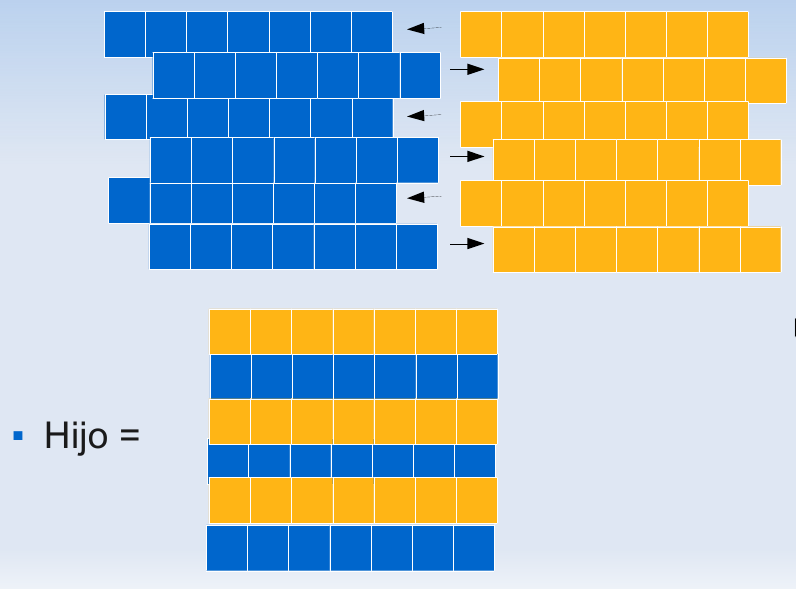
\includegraphics[scale=0.2]{cross.png}
\caption{Operador de Crossover}
\end{figure}

El operador de Crossover realiza un cruce por filas de dos cromosomas dados. Del primer padre toma las filas pares y del segundo la filas impares, y a partir de ellas genera un nuevo hijo, que gracias a la representaci\'on que se realiz\'o, permite siempre obtener soluciones factibles.

\begin{figure}[htp]
\centering
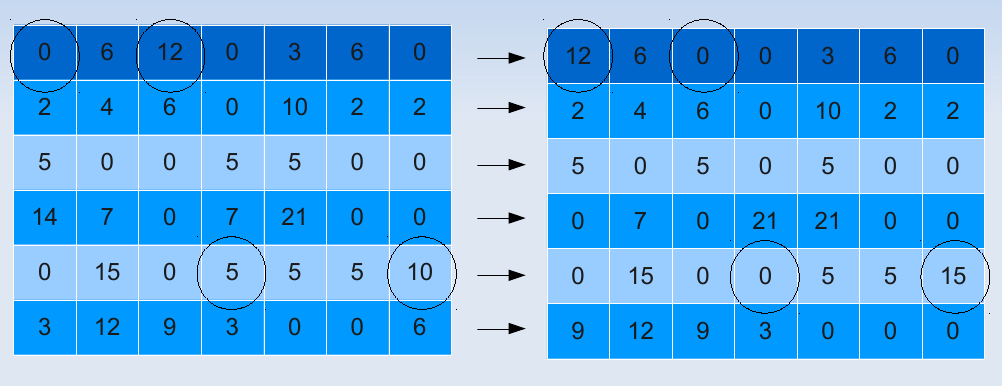
\includegraphics[scale=0.2]{mut.png}
\caption{Operador de Mutaci\'on}
\end{figure}

El operador de mutaci\'on se ejecuta con una probabilidad de 0.3, y cuando se ejecuta selecciona aleatoriamente el n\'umero de hijos que se mutaran. Y el efecto que tiene es que para cada fila del cromosoma, correspondiente a un cliente, realiza el equivalente a mover un grupo entero de piezas de una columna a otra, de igual manera aleatoriamente. En el ejemplo de la figura 5 queda mejor reflejado.


\begin{verbatim}
class Chromosome {

  int **genes;
  int quality;
  int req;
  int width;
  int *tops;
  int heightMax;
  int area;
  int lines;

  Chromosome(int, int);
  ~Chromosome();  
  void updateQuality();
  Chromosome* crossover(Chromosome*);
  void mutation();
  void fillChrom(int*, int*);
  void print();
};
\end{verbatim}

\newpage

\subsubsection{Algoritmo de Colonia de Hormigas}

Para entender el algoritmo de hormigas que hemos implementado restringiremos la altura maxima 
que nuestros patrones pueden tener por $L$ fijo y seguidamente indexemos el conjunto de las piezas de $1$ hasta $n$, 
con $n$ igual al total de piezas distintas:

\begin{definicion}
Definiremos las variables $l_i$ como la longitud de la pieza $i$
\end{definicion}

\begin{definicion}
Una columna factible es un multiconjunto de enteros $\{i_1 ,i_2 ,\dots ,i_h\}$ tales que $\Sigma _{k=1}^h l_{i_k}\leq L$.
\end{definicion}

Dado un numero de tipos de piezas fijas y sus respectivas longitudes, se tiene que el n\'umero 
total de columnas factibles es finito, denotemos a este n\'umero finito por $m$ e indexemos el conjunto de columnas 
factibles.

\begin{definicion}
Sea $\{i_1 ,i_2,\dots ,i_h\}$ la columna factible $j$, denotemos entonces por $S_i$ como el n\'umero $L-\Sigma _{k=1}^h l_{i_k}$ 
y a $O_{ij}$ como la cantidad de veces que se repite el entero $i$ en la columna factible $j$ 
\end{definicion}

A continuaci\'on describiremos el algoritmo:

El concepto de columna factible es fundamental para nuestro algoritmo de hormigas, por lo tanto es importante destacar que representaremos 
una columna factible $j$ como un arreglo de enteros de tama\~no igual al total de piezas distintas y donde cada entero 
ser\'a un $O_{ij}$.

La primera etapa del algoritmo consiste en calcular todas las posibles columnas factibles y colocar cada una de ella en un 
arreglo, de modo que este arreglo implementa la indexaci\'on necesaria que se mensionaba en los p\'arrafos anteriores para poder definir 
las variables $S_j$ y $O_{ij}$.

La idea del algoritmo es que en cada iteraci\'on, cada hormiga escoja probabilisticamente una columna factible hasta el punto que el 
total de las piezas de todas estas columnas sobrepase el total de las piezas del problema. El exeso de piezas ser\'a penalizado en la 
funci\'on objetivo y las probabilidades de escogencia de columna ser\'a menor en la medida que de estas escogencias resulte un crecimiento del n\'umero 
extras de piezas.

La funci\'on objetivo seg\'un lo dicho anteriormente ser\'a $\Sigma _{j=1}^m S_jX_j+\Sigma _{i=1}^n V_i$ donde $X_i$ es el n\'umero de veces 
que se us\'o la columna factible $j$ en la soluci\'on y $V_i$ es el total de las piezas extras.

Las probabilidades de escogencia de las columnas se realizan en dos etapas: Primero se escoje una pieza probabilisticamente y luego se escoje 
(probabilisticamente tambien) una columna donde se encuentre la pieza escojida.

Para asignar las probabilidades antes mencionadas necesitamos la siguiente.

\begin{definicion} 
Para una soluci\'on (no necesariamente factible) fija definimos a $P_i$ como la cantidad de piezas del tipo $i$ que se encuentran en dicha 
soluci\'on y a $D_i$ como la cantidad m\'axima de piezas disponibles del tipo $i$
\end{definicion}

\begin{definicion}
$$M_i:=\left\{\begin{array}{lcc}
              D_i-P_i & si & P_i> 0 \\
             \\ 0   & si & D_i-P_i\leq 0
             \end{array}
      \right.  $$
\end{definicion}

\begin{definicion}
Denotaremos por $TM$ a la suma $\Sigma _{\forall i} M_i$
\end{definicion}

En la primera iteraci\'on de nuestro algoritmo la probabilidad de escoger la pieza $i$ ser\'a igual a $\frac{M_i}{\Sigma _{\forall k}M_k}$ y una 
vez escogida $i$ la probabilidad de escoger una columna factible $j$ que contenga la pieza $i$ ser\'a $1-\frac{S_j}{\Sigma _{k\in \Omega _i}S_k}$, 
donde $\Omega _i:=\{j|O_{ij}>0\}$.

Como es posible con estas probabilidades que se obtenga una soluci\'on no factible con mayor cantidad de piezas de alg\'un tipo de la permitida, 
entonces en las siguientes iteraciones las probabilidades penalizan estas situaciones. Para definir estas probabilidades necesitamos las siguientes 

\begin{definicion}
Denotaremos por $P'_i$ el n\'umero total de piezas de la soluci\'on de la iteraci\'on anterior y definamos $$V'^{aux}_i:=(P'_i-D_i)*l_i$$
\end{definicion}

No nos interesa que $V'^{aux}_i=0$ y que piezas que no tiene una cantidad execiva en la iteraci\'on anterior tenga mucha mas probabilidad de 
escogerce que otras, de esta forma damos valores mas uniformes de $V'$ en la siguiente

\begin{definicion}
$$V'_i:=\left\{\begin{array}{lcc}
              V'^{aux}_i & si & V'^{aux}_i> 0 \\
             \\ (0.5)min\{V'^{aux}_j|V'^{aux}_j>0\}   & si & V'^{aux}_i=0
             \end{array}
      \right.  $$
\end{definicion}

\begin{definicion}
Denotemos por $TOV'$ a $\Sigma_{\forall i}V'_i$
\end{definicion}

De esta forma la probabilidad de escogencia de la pieza $i$ para iteraciones distintas a la primera es $\frac{\frac{M_i}{TM}(1-\frac{V'_i}{TOV'})}{Sum}$
donde $Sum=\Sigma _{\forall i} \frac{M_i}{TM}(1-\frac{V'_i}{TOV'})$, y por lo tanto mientras mas se sobrepase la cantidad de piezas del tipo $i$ en la 
soluci\'on de la iteraci\'on anterior, menos probabilidad tiene de ser escogida en la actual iteraci\'on.

Una vez que se escoge la pieza $i$ las probabilidades para escoger una columna factible $j$ es $\frac{P'_j}{\Sigma _{\forall j\in \Omega _i}P'_j}$ 
con $\Omega _i =\{j|\forall O_{ij}>0\}$ y $P'_j$ dada por la siguiente definici\'on

\begin{definicion}
Sean $X_{0(k)}$ y $X_{0(k-1)}$ los valores de la funci\'on objetivo de la soluci\'on de la iteraci\'on $k$ y $k-1$ (suponemos que la iteraci\'on 
actual es la $k+1$) respectivamente, y sea $N'_j$ el n\'umero de veces que se escogio la columna factible $j$ en la soluci\'on de la 
iteraci\'on anterior, entonces 
definimos:
$$P'_j:=\left\{\begin{array}{lcc}
              \frac{1}{N'_jS_j}O_{ij} & si &  X_{0(k)}> X_{0(k-1)}\\
             \\ \frac{N'_j}{S_j}O_{ij}   & si X_{0(k)}\leq X_{0(k-1)}& 
             \end{array}
      \right.  $$
\end{definicion}

Esta escogencia del valor de $P'_j$ en funci\'on de si las soluciones mejoran o no en cada iteraci\'on es una simulaci\'on de la evaporaci\'on 
de la feromona.

\newpage

\subsection{Representaci\'on de la soluci\'on}

La soluci\'on al problema de CSP se encuentra representada mediante la clase \emph{Pattern}, en donde se encuentra 
una lista de piezas que fueron cortadas y poseen mediante la clase \emph{Piece} una serie de atributos que denotan
la posici\'on en la tela, y forman el patr\'on como fue cortada. Adem\'as podemos saber la altura y el n\'umero de lineas 
creadas con el corte, y analizar una funci\'on objetivo.\\

Esto es de manera general, pero la estructura que en concreto representar\'a nuestra soluci\'on se basa en un arreglo de
listas de piezas. El tamaño del arreglo viene definido por el ancho fijo de la tela a cortar, y cada una de las listas
se compone por la piezas colocadas al estilo de una pila, en la columna \emph{i} del arregla o tela. Esta representaci\'on
nos ser\'a de conveniencia al momento de realizar un movimiento para generar un estado vecino.

\subsection{Funci\'on Objetivo}

La funci\'on objetivo que vamos a utilizar esta definida por diferentes par\'ametros. De manera general definimos
una m\'etrica de calidad de los estados soluci\'on basada en la m\'axima altura generada por el corte de cada una de las piezas.
Es decir que si comparamos dos estados soluci\'on, en donde ambos tengan un patr\'on con el mismo n\'umero de piezas cortadas, 
es decir, la misma \'area ocupada, aquel patr\'on que tenga la altura menor sera la mejor. 
Indirectamente al hablar de altura m\'inima, esto se refiere a el m\'inimo de \'area o material desperdiciado.
En primera instancia esa es la m\'etrica que vamos a utilizar en nuestro problema.\\

Otra funci\'on objetivo que podemos usar esta basada en el n\'umero de lineas completas generadas en el patr\'on, es decir,
todas las lineas completas de que tengan el ancho total de la tela, y como altura una unidad. El problema de esta m\'etrica es que podemos encontrar dos patrones con el mismo n\'umero de lineas, pero con alturas muy diferente, en donde el malgasto sea excesivo.\\

Una idea mejor es crear una funci\'on objetivo que relacione las dos m\'etricas anteriores, aunque actualmente no 
hemos definido esta estrategia para ser usada en las metaheuristicas a implementar.

\subsection{Operadores}

Al inicio del proyecto, para generar la vecindad para un estado soluci\'on utilizabamos un conjunto de tres operadores, basados en el movimiento de piezas. El operador
de primer nivel genera una vecindad moviendo una pieza seleccionada de los niveles superiores. El siguiente operador, de segundo nivel, fija una pieza seleccionada y realiza una llamada recursiva al operador de primer nivel, al final se recolocar\'a la pieza fijada, resultando asi un movimiento de dos piezas. El tercer operador es una llamada al operador de tercer nivel, en donde se fija una pieza y se llama a el operador de segundo nivel.\\

Pero al analizar estos operadores nos dimos cuenta que resultaban ineficientes y la vecinandad que generaban era excesivamente grande. Por lo tanto, siguiendo recomendaciones
de compa\~neros de clase, decidimos implementar un nuevo operador. Este nuevo operador se basa en mover cualquier pieza seleccionada entre todo el conjunto, a alguna posici\'on
en el tope del patr\'on de corte. De esta manera el tama\~no de la vecindad ser\'a siempre finita, definida por $$ V =  (\sum_{i = 1}^{N} L_i) \times W $$ que es solo multiplicar
el n\'umero total de piezas por el ancho fijo de la tela. Entonces para aquellas metaheur\'isticas donde sea necesario generar toda una vecindad, en general el uso de memoria
sera siempre fijo, y la diversidad de los patrones sera considerable.

\newpage

\section{Detalles de implementaci\'on}

\subsection{Pseudoc\'odigo de las Metaheur\'isticas}

\subsubsection{Algoritmo de Local Search}

\begin{algorithmic}

\REQUIRE Patron inicial : initial

\STATE $k \gets 0$
\STATE  Patron $actual \gets initial$
\STATE  Patron $next$
\STATE  Lista Patrones $vicinity$

\WHILE{ $k < 50$ }
	\STATE $ vicinity \gets actual.genVicinity() $
	\WHILE {$ !vicinity.empty() $}
		\STATE $next = v$
      	\IF {$ (next.quality() < actual.quality() $}
        	\STATE $actual.destroy() $
        	\STATE $ actual \gets next$
        	\STATE $break$
        \ENDIF
    \ENDWHILE
    \STATE $k++$
    \STATE $deleteList(vicinity)$
\ENDWHILE
\RETURN  return actual;

\end{algorithmic}

\subsubsection{Algoritmo de Local Search - Mejor Mejor}

\begin{algorithmic}

\REQUIRE Patron inicial : initial

\STATE $k \gets 0$
\STATE  Patron $actual \gets initial$
\STATE  Patron $next \gets actual$
\STATE  Lista Patrones $vicinity$

\WHILE{ $k < 50$ }
	
	\STATE $ best \gets actual $
	\STATE $ vicinity \gets actual.genVicinity() $
	\WHILE {$ !vicinity.empty() $}
		\STATE $next = v$
      	\IF {$ (next.quality() < best.quality() $}
        	\STATE $actual.destroy() $
        	\STATE $ best \gets next$
        \ENDIF
    \ENDWHILE
   	\IF {$ (best.quality() < actual.quality() $}
       	\STATE $actual.destroy() $
       	\STATE $ actual \gets best$
	\ENDIF
    \STATE $k++$
    \STATE $deleteList(vicinity)$
\ENDWHILE
\RETURN  return actual;

\end{algorithmic}

\subsubsection{Algoritmo de ILS}

\begin{center}
\begin{algorithmic}

\REQUIRE Patron inicial: $s_{mejor}$

\STATE $k \gets 0$
\STATE Patron $s1$,$s2$
\STATE Patron $s_{mejor} \gets localSearch(s_{mejor})$

\WHILE {$ k < 10 $}
    \STATE $ s1 \gets s_{mejor}.perturbar() $
    \STATE $ s2 \gets localSearch(s1) $
    \IF {$ s2.quality() < s_{mejor}.quality()$ }
    	\STATE $ s_{mejor}.destroy() $
        \STATE $ s_{mejor} \gets s2 $
    \ENDIF
    \STATE $ s2.destroy() $
    \STATE $k++$
\ENDWHILE
\RETURN $s_{mejor}$

\end{algorithmic}
\end{center}

\subsubsection{Algoritmo de GRASP}

\begin{center}
\begin{algorithmic}

\REQUIRE Lista Piezas $piecesPart$, int $demanda$
\STATE  Patron $pat$
\STATE  Lista Patron $RCL$
\STATE  int $ran$, $count$
  
\WHILE {$i < demanda$}
	\WHILE {$j < 20$}
    	\STATE $RCL.insert(pat.addRequest(piecesPart[i]))$
    \ENDWHILE
    \STATE $RCL.sort()$
    \STATE $ran \gets random()$
    \STATE $count \gets 0$

    \WHILE {$!RCL.empty()$}
    	\STATE $count++$
      	\IF {$count = ran$}
        	\STATE $pat.destroy()$
        	\STATE $pat \gets RCL(r)$
        	\STATE $break$
      	\ENDIF
    \ENDWHILE
   
    \STATE $pat \gets localSearch(pat)$
\ENDWHILE
\RETURN $pat$

\end{algorithmic}
\end{center}

\subsubsection{Algoritmo de Simulated Anneling}

\begin{center}
\begin{algorithmic}

\REQUIRE Patron $Initial$

\STATE int $i \gets 0$

\STATE int $a \gets 0$
\STATE int $maxAccept \gets 20$  

\STATE double $k \gets 0.0$
\STATE double $maxIter \gets 200.0$
\STATE double $ro \gets 1.05$

\STATE double $temp \gets 1000.0$
\STATE double $alfa \gets 0.8$

\STATE double $delta$
\STATE int $from, pieceNum, to$
\STATE double $suerte$
  
\STATE Patron $actual \gets initial.clone()$
\STATE Patron $next$

\WHILE {$i < 50$}

	\WHILE {$k < maxIter \wedge a < maxAccept$}

		\WHILE {$true$}
        	\STATE $from \gets random(1,width)$
        	\IF {$actual.pieces[from].size() != 0$}
          		\STATE $pieceNum \gets random(0,numPiecesFrom)$
          		\STATE $to \gets random(1,width)$
          		\STATE $break$
        	\ENDIF
      	\ENDWHILE

      	\COMMENT {Se genera el vecino proximo a evaluar}
      	\STATE $next \gets actual.vicinityOperator(from,pieceNum,to)$

      	\COMMENT {Se calcula el delta con la comparacion de calidades}
      	\STATE $delta \gets next.quality() - actual.quality()$

      	\IF {$delta < 0$}	
        	\STATE $actual.destroy()$
        	\STATE $actual \gets next.clone()$
        	\STATE $a++$	
      	\ELSE
        	\STATE $suerte \gets random(0,1)$
        	\IF {$temp > 0.0$}
          		\IF { $suerte < e^{-delta/temp}$} 
            		\STATE $actual.destroy()$
            		\STATE $actual \gets next.clone()$
            		\STATE $a++$
          		\ENDIF
        	\ENDIF
      	\ENDIF

      	\STATE $k \gets k + 1$
    \ENDWHILE
    
 	\COMMENT {Disminuye la temperatura}
    \STATE $temp \gets temp * alfa$
    \COMMENT {Aumenta el numero de iteraciones}
    \STATE $maxIter \gets maxIter * ro$
    \STATE $k \gets 0.0$
    \STATE $a \gets 0$
    \STATE $i++$
\ENDWHILE
  
\RETURN actual;

\end{algorithmic}
\end{center}

\subsubsection{Algoritmo Gen\'etico}

\begin{center}
\begin{algorithmic}

\REQUIRE int $request$, int $width$, int[] $numPieces$, int[] $largePieces$

\STATE int $sizePop \gets 400$
\STATE Lista de Cromosomas $population$, $best$, $worst$, $child$
\STATE Iterador sobre lista de Cromosomas $it$, $itB$, $itW$
\STATE Iterador reverso sobre lista de Cromosomas $rit$
\STATE Cromosoma $ch$
\STATE int $count \gets 0$
\STATE double $suerte$
\STATE double $probMut \gets 0.3$
\STATE int $ran$
\\
\COMMENT {Se genera la Poblacion inicial}

\WHILE {$i < sizePop$}
	\STATE $ch \gets new Chromosome(request,width)$
    \STATE $ch.fillChrom(numPieces,largePieces)$
    \STATE $population.insert(ch)$
    \STATE $i++$
\ENDWHILE

\WHILE {$g < 1000$}

    \STATE $population.sort()$
	\COMMENT {Se ordena la poblacion por calidad}  
  
    \COMMENT {Se toman los mejores}
    \STATE $count \gets 0$
    \WHILE {$count < sizePop/4$}
    	\STATE $it \gets population.getBest()$
    	\STATE $best.insert(it)$
    \ENDWHILE

    \COMMENT {Se toman los peores}
    \STATE $count \gets 0$
    \WHILE {$count < sizePop/4$}
    	\STATE $it \gets population.getWorst()$
    	\STATE $worst.insert(it)$
    \ENDWHILE

    \COMMENT {Se cruzan los mejores con los peores}
    \STATE $count \gets 0$
    \WHILE {$count < sizePop/4$}
    	\STATE $itB \gets population.getBest()$
		\STATE $itW \gets population.getWorst()$
    	\STATE $child.insert(croosover(itB,itW))$
    \ENDWHILE

    \COMMENT {Se cruzan los mejores entre ellos}
    \STATE $count \gets 0$
    \WHILE {$count < sizePop/4$}
    	\STATE $itB1 \gets population.getBest()$
		\STATE $itB2 \gets population.getAnotheBest()$
    	\STATE $child.insert(croosover(itB1,itB2))$
    \ENDWHILE

    \COMMENT {Se decide si se realiza mutacion}
    \STATE $suerte \gets random(0,1)$
    \IF {$suerte < probMut$}
    	\STATE $ran \gets random(1,sizeChild)$
      	\STATE $count \gets 0$
		\WHILE {$count < ran$}      
			\STATE $it \gets child.get()$
			\STATE $it.mutation()$	
		\ENDWHILE
	\ENDIF

    \COMMENT {Se realiza la repoblacion}
    \STATE $count \gets 0$
    \WHILE {$count < child.size()$}
	    \STATE $itW \gets population.getWorst()$
      	\STATE $population.erase(itW)$
		\STATE $it \gets child.get()$
		\STATE $population.insert(it)$	
    \ENDWHILE
    
\ENDWHILE

\STATE $population.sort()$
  
\RETURN $population.front()$

\end{algorithmic}
\end{center}

\section{Instrucciones de operaci\'on}

Para compilar el programa debe realizar la llamada:
\begin{verbatim}
    $> make
\end{verbatim}
Y para realizar la corrida:
\begin{verbatim}
    $> ./CSP Metaheuristica Instancia -- Ej: ./CSP ILS 100
\end{verbatim}

\section{Experimentos y an\'alisis de resultados}

En la siguiente seccion detallaremos cuales fueron las instancias que fueron corridas, y un analisis de las
diferentes metaheuristicas que fueron implementadas.

\subsection{Instancias}

En la literatura y en las librerias en la red, se nos fue imposible encontrar un set de problemas para correr
nuestros algoritmos. En general tuvimos que dise\~nar nuestros propios casos de prueba, los cuales se listan a continuacion en un formato definido como un vector $\lbrace C_1/L_1, C_2/L_2, ... , C_n/L_n\rbrace$, donde cada $C_i$ representa la cantidad de bloques de tama\~no $L_i$:

\begin{enumerate}
\item Instancia de 55 piezas: tela de 10 de ancho con de 8 clientes con la siguiente demanda: $\lbrace3/8,5/4,7/6,9/2,5/8,15/5,6/9,5/7\rbrace$
\item Instancia de 66 piezas: tela de 8 de ancho con de 7 clientes con la siguiente demanda: $\lbrace7/6, 5/2, 11/3, 20/5, 5/2, 8/5, 10/4\rbrace$
\item Instancia de 100 piezas: tela de 8 de ancho con de 5 clientes con la siguiente demanda: $\lbrace20/5, 20/4, 20/3, 20/2, 20/7\rbrace$
\item Instancia de 150 piezas: tela de 10 de ancho con de 14 clientes con la siguiente demanda: $\lbrace13/8, 5/4, 17/6, 9/2, 15/8, 15/5, 6/9, 5/7, 10/2, 24/8, 8/7, 9/9, 10/2, 4/10 \rbrace$
\end{enumerate}

\subsection{Resultados y analisis de las Metaher\'isticas}

Como se ha mencionado a lo largo del informe, las metaheur\'isticas que fueron implementadas y corridas fueron las de trayectoria LS, LS-MM, ILS y Simulated Anneling, las constructivas de GRASP y Hormiga y finalmente un algoritmo Gen\'etico en la parte de poblacionales.\\

En general las corridas de los diferentes algoritmos generaban buenos resultados, a excepci\'on de algunos que ofrecian normalmente malas soluciones, o aquellos algoritmos mas estables que generalmente ofrecian buenas soluciones. Para los algoritmos de trayectoria se obtiene un mejor resultado para Simulated Anneling, el cual result\'o ser el que mejor se adapta al problema y ofrece los optimos para todas las instancias. Con relaci\'on a los de b\'usqueda, solo la b\'usqueda local iterada (ILS) logro obtener buenos resultados, pero adicionando un costo de tiempo y memoria que pueden resultar vitales. Para la b\'usqueda local sencilla lo mas importante es la dependencia con la soluci\'on inicial, en general para una soluci\'on inicial ``buena'' el algoritmo se quedaba en un optimo local, pero al realizar una gran perturbaci\'on a la misma, y obtener una soluci\'on inicial ``peor'', el algoritmo lograba converger a una mejor soluci\'on cerca del optimo del problema.\\

Para los algoritmos constructivos no pudimos obtener buenos resultados. Especificamente para la metaheur\'istica de GRASP no fue posible encontrar una soluci\'on buena que se acercara al optimo de la instancia. La opci\'on constructiva no aporta un beneficio para esta clase de problema, porque aunque se elijan los mejores siempre de una lista de candidatos, la soluci\'on greedy te va adaptando el problema a una convergencia siempre a un optimo local, a veces definido en la etapa de optimizaci\'on del algoritmo.\\

Otros buenos resultados se obtuvieron del algoritmo Gen\'etico, el cual gracias a la representaci\'on realizada permiti\'o diversificar mucho el espacio de resultados que se pueden obtener, y con los operadores de cruce y mutacion fue posible ir generando nuevas generaciones de soluciones factibles que por lo general siempre lograban converger a una buena soluci\'on.

\section{Estado actual}

\subsection{Estado final de la aplicaci\'on}

La aplicaci\'on se encuentra totalmente operativa con relaci\'on a la representaci\'on del problema, una soluci\'on
factible, los operadores y la funci\'on objetivo. Adem\'as estan implementadas y funcionales las metaheur\'isticas de LS, LS-MM, ILS, GRASP, Simulated Anneling y Algoritmo Gen\'etico. Y aunque se realiz\'o una implementaci\'on de  Hormiga, no se encuentra del todo operativa.	

\newpage

\section{Conclusiones y recomendaciones}

En el desarrollo de esta tercera etapa del proyecto pudimos reafirmar la complejidad que tiene este problema
en cuanto a su representaci\'on, y de la cual depende en gran cabida el funcionamiento de las diferentes 
metaheur\'isticas. Sin embargo, fue posible solventar los diferentes problemas que encontramos en la 2da entrega,
y ahora tenemos una representaci\'on s\'olida y m\'as f\'acil de utilizar, la cual consigui representar de manera efectiva el problema que estamos atacando.\\

Ya para finalizar pudimos determinar que son dos metaheuristicas las que mejor se adecuan a nuestro problema y que ofrecen buenas soluciones en un tiempo reducido y con poca necesidad de recursos computacionales. Las mismas fueron la metaheur\'istica de trayectoria Simulated Anneling, que es la mas estable de todas, en donde para toda corrida siempre ofrece muy buenos resultados iguales o cercanos al optimo de la instancia. Y por otro lado el Algoritmo Gen\'etico, que para soluciones peque\~nas y medianas resulta ser bastante estable y genera buenas soluciones. Con un detalle, que para problemas mas grandes se deben realizar algunas adaptaciones, aunque sigue teniendo un mejor desempe\~no que otras metaheur\'isticas probadas.

\newpage

\section{Referencias bibliogr\'aficas}

\begin{thebibliography}{99}
  
\bibitem[1]{ref:steel}
  \textbf{Solving the Cutting Stock Problem in the Steel Industry}\\
  \textit{KARELAHTI J.}

\bibitem[2]{ref:genetic}
  \textbf{A Genetic Solution for the Cutting Stock Problem}\\
  \textit{ANDRAS P., ANDRAS A, SZABO Z.}

\bibitem[3]{ref:prog}
  \textbf{A Progressive Heuristic Search for the Cutting Stock Problem}\\
  \textit{ONAINDIA E., BARBER F., BOTTI V., CARRASCOSA C., HERNANDEZ M., REBOLLO M.}

\bibitem[4]{ref:aco}
  \textbf{An ACO Algorithm for One-Dimensional Cutting Stock Problem}\\
  \textit{ESHGHI K., JAVANSHIR H.}
  
\bibitem[5]{ref:genetic2}
  \textbf{Using Genetic Algorithms in Solving the One-Dimensional Cutting Stock Problem in the Construction Industry}\\
  \textit{SHAHIM A., SALEM O.}
  
\bibitem[6]{ref:simulated}
  \textbf{A Simulated Aneeling Approach for a Standard One-Dimensional Cutting Stock Problem}\\
  \textit{JAHROMI M.H.M.A., TAVAKKOLI-MOGHADDAM R., GIVAKI E., REZAPOUR-ZIBA A.}
  
\bibitem[7]{ref:aco}
  \textbf{An ACO Algorithm for One-Dimensional Cutting Stock Problem}\\
  \textit{ESHGHI K., JAVANSHIR H.}

  \end{thebibliography}
  
\end{document}
